\chapter{प्लाज़्मा, चालक और परावैद्युत में विद्युत्चुंबकीय तरंगें}\label{ch:b2:waves-in-media}

कोई लघुतरंग प्रसारण ऊपरी वायुमंडल से टकराकर किसी महासागर को पार कर
जाता है, क्योंकि वह परत उसे दर्पण की तरह लौटा देती है --- फिर भी वही परत
दूरदर्शन और उपग्रह-संकेतों को पार जाने देती है। धातु का चम्मच चमकीला है,
सूक्ष्मतरंग-भट्ठी के दरवाज़े की धातु-जाली तरंगों को भीतर रोके रखती है जबकि
आप उसमें से अपना भोजन देखते रहते हैं, और काँच की एक शीट प्रकाश के लिए
पारदर्शी है पर पराबैंगनी के लिए अपारदर्शी। हर हाल में कोई तरंग किसी
पदार्थ में घुसती है, पदार्थ के आवेश उत्तर देते हैं, और उनका उत्तर तरंग को
बदल देता है: उसकी चाल, उसका \omterm{def:b2:dispersion-wave-packets:complex}{क्षीणन}, यहाँ तक कि वह चलती भी है या नहीं।
यह अध्याय किसी माध्यम के तीन मानक प्रतिरूप लेता है --- मुक्त इलेक्ट्रॉनों की
कोई गैस, कोई ओमीय चालक, और बद्ध इलेक्ट्रॉन --- उसी एक विधि के साथ जो
तीनों को सँभाल लेती है: प्रेरित धारा को \omterm{thm:b2:maxwell-equations:maxwell}{मैक्सवेल के समीकरणों} में जोड़िए और
परिक्षेपण-संबंध पढ़ लीजिए।

\section{प्लाज़्मा में तरंगें}

\begin{definition}[प्लाज़्मा; मुक्त-इलेक्ट्रॉन प्रतिरूप]\label{def:b2:waves-in-media:plasma}
\index{प्लाज़्मा}\index{प्लाज़्मा आवृत्ति}
कोई \emph{प्लाज़्मा} मुक्त इलेक्ट्रॉनों (घनत्व
$n$, द्रव्यमान $m$, आवेश $-e$) और धनायनों की समग्र रूप से उदासीन कोई गैस
है, और आयन, हज़ारों गुना भारी होने के कारण, स्थिर मान लिए जाते हैं। ऊपरी
वायुमंडल (आयनमंडल, $n \sim 10^{11}$--$10^{12}$ m$^{-3}$), कोई विसर्जन नलिका,
सौर किरीट, और --- प्रकाशिक आवृत्तियों पर --- किसी धातु के चालन इलेक्ट्रॉन
प्लाज़्मा हैं। टक्करें उपेक्षित हैं (तरंग का आवर्तकाल दो टक्करों के बीच के
समय की तुलना में छोटा है)। इसकी अभिलाक्षणिक आवृत्ति है
\emph{प्लाज़्मा आवृत्ति}
\[
\omega_p = \sqrt{\frac{ne^2}{\varepsilon_0m}} , \qquad
f_p = \frac{\omega_p}{2\pi} \approx 9\,\text{Hz}\times\sqrt{n\,[\text{m}^{-3}]} :
\]
आयनमंडल के लिए \qty{3}{MHz} से \qty{9}{MHz} तक, और किसी धातु के लिए
\qty{2e15}{Hz} (पराबैंगनी)।
\end{definition}

\begin{theorem}[प्लाज़्मा का परिक्षेपण-संबंध]\label{thm:b2:waves-in-media:plasmadispersion}
\index{कटाव आवृत्ति (प्लाज़्मा)}\index{क्षयी तरंग (प्लाज़्मा)}
किसी \omterm{def:b2:waves-in-media:plasma}{प्लाज़्मा} में किसी अनुप्रस्थ PPH तरंग $\underline{\vect E} = \underline{\vect E}_0\eu^{\iu(\omega t - kx)}$ के
लिए इलेक्ट्रॉन $\underline{\vect v} = -e\underline{\vect E}/\iu m\omega$ से दोलन करते हैं
और धारा-घनत्व $\underline{\vect j} = \underline\gamma\underline{\vect E}$ ले चलते हैं, जिसमें
$\underline\gamma = ne^2/\iu m\omega$; तब \omterm{thm:b2:maxwell-equations:maxwell}{मैक्सवेल के समीकरण} देते हैं
\[
k^2 = \frac{\omega^2 - \omega_p^2}{c^2} .
\]
$\omega_p$ के ऊपर तरंग चलती है, जिसमें $v_\varphi = c/\sqrt{1 - \omega_p^2/\omega^2}
> c$ और $v_g = c\sqrt{1 - \omega_p^2/\omega^2} < c$, $v_\varphi v_g = c^2$; $\omega_p$ के
नीचे $k = -\iu\kappa$, जहाँ $\kappa = \sqrt{\omega_p^2 - \omega^2}/c$: तरंग
\emph{क्षयी} है, $1/\kappa$ जितना ही घुस पाती है और पूरी तरह परावर्तित हो जाती है
(\cref{ch:b2:wave-interfaces}); तब \omterm{def:b2:waves-in-media:plasma}{प्लाज़्मा} कोई दर्पण है। $\omega
\gg \omega_p$ पर इलेक्ट्रॉन साथ नहीं दे पाते और \omterm{def:b2:waves-in-media:plasma}{प्लाज़्मा} पारदर्शी है।
\end{theorem}

\begin{proof}
गति-समीकरण $m\,\dd\vect v/\dd t = -e\vect E$ (चुंबकीय बल
$ev B \sim evE/c$ $v \ll c$ के लिए नगण्य है, और आयनों की गति
$m/M$ गुना छोटी है): $\iu m\omega\underline{\vect v} = -e\underline{\vect E}$। फिर
$\underline{\vect j} = -ne\underline{\vect v}$। किसी अनुप्रस्थ तरंग के लिए \omterm{def:b2:waves-in-media:plasma}{प्लाज़्मा} उदासीन बना रहता
है ($\vect k\cdot\vect E = 0$ गाउस से $\rho = 0$ देता है), अतः
मैक्सवेल--ऐंपियर बनता है $-\iu\vect k\wedge\underline{\vect B} = \mu_0\underline\gamma\underline{\vect E}
+ \iu\omega\mu_0\varepsilon_0\underline{\vect E}$ और मैक्सवेल--फ़ैराडे $\underline{\vect B} = \vect k
\wedge\underline{\vect E}/\omega$; जोड़ने पर, $k^2\underline{\vect E} = \mu_0(\iu\omega\underline\gamma -
\omega^2\varepsilon_0)(-1)\underline{\vect E}$, अर्थात् $k^2 = \omega^2\mu_0\varepsilon_0 - \iu\omega\mu_0
\underline\gamma = (\omega^2 - ne^2/\varepsilon_0m)/c^2$। वेग वैसे ही निकलते हैं जैसे
\cref{ch:b2:dispersion-wave-packets} में।
\end{proof}

\begin{remark}[ऊर्जा कहाँ जाती है]\label{rem:b2:waves-in-media:plasmaenergy}
चालकता काल्पनिक है: $\langle\vect j\cdot\vect E\rangle = 0$, अर्थात् इलेक्ट्रॉन
आधे चक्र में तरंग से ऊर्जा लेते हैं और अगले आधे में लौटा देते हैं --- कोई
हानिरहित माध्यम, जिसमें तरंग की ऊर्जा क्षेत्रों और इलेक्ट्रॉनों की गतिज
ऊर्जा के बीच बँटी रहती है, और $v_g$ से चलती है। टक्करें $\underline\gamma$ में कोई
छोटा वास्तविक भाग और कोई छोटा अवशोषण जोड़ देती हैं: आयनमंडल की D परत
दिन में मध्यम तरंगों को सोख लेती है, और इसीलिए दूर के AM केंद्र रात में
सुनाई देते हैं।
\end{remark}

\begin{example}[आयनमंडल और रेडियो]\label{ex:b2:waves-in-media:ionosphere}
F परत में $n = \qty{1e12}{m^{-3}}$ लेने पर $f_p = \qty{9}{MHz}$: उससे नीचे के
लघुतरंग प्रसारण परावर्तित होते हैं (और आयनमंडल तथा ज़मीन के बीच उछलते हुए
पृथ्वी का चक्कर लगा सकते हैं), जबकि FM (\qty{100}{MHz}), दूरदर्शन
और उपग्रह-कड़ियाँ पार निकल जाती हैं। \qty{3}{MHz} की कोई तरंग परत में लौट पड़ने
से पहले केवल $1/\kappa = c/\sqrt{\omega_p^2 - \omega^2} = \qty{6}{m}$ तक घुसती है।
वायुमंडल में लौटता कोई अंतरिक्ष-यान $n \sim 10^{18}$ m$^{-3}$,
$f_p \sim \qty{10}{GHz}$ के \omterm{def:b2:waves-in-media:plasma}{प्लाज़्मा} में लिपट जाता है: रेडियो संपर्क मिनटों तक टूट जाता है।
\end{example}

\begin{omfigure}
\begin{tikzpicture}
\begin{axis}[omaxis, axis x line=bottom, axis y line=left, width=6.2cm, height=4.6cm,
    xlabel={$kc/\omega_p$}, ylabel={$\omega/\omega_p$}, xmin=0, xmax=3, ymin=0, ymax=3.3, xtick={1,2,3}, ytick={1,2,3}, samples=80,
    xlabel style={at={(axis description cs:0.5,-0.12)}, anchor=north},
    ylabel style={at={(axis description cs:-0.12,0.5)}, rotate=90, anchor=south},
    legend style={font=\scriptsize, at={(0.97,0.05)}, anchor=south east, draw=none, fill=none}]
  \addplot[omThm, thick, domain=0:3] {sqrt(1+x*x)};
  \addplot[omDef, dashed, domain=0:3] {x};
  \addplot[black, dotted] coordinates {(0,1) (3,1)};
  \legend{प्लाज़्मा, $\omega = ck$}
  \node[font=\scriptsize, anchor=west] at (axis cs:0.1,0.5) {क्षयी};
\end{axis}
\end{tikzpicture}
\hfill
\begin{tikzpicture}[font=\small, x=1cm, y=1cm, >=Stealth]
  \draw[thick] (-3.4,0) -- (3.4,0); \node[font=\footnotesize] at (2.9,-0.3) {ज़मीन};
  \draw[omExo, thick, dashed] (-3.4,2.6) -- (3.4,2.6); \node[omExo, font=\footnotesize] at (2.6,2.85) {आयनमंडल, $n_e$};
  \draw[omThm, thick, ->] (-3.0,0) -- (-1.5,2.55); \draw[omThm, thick, ->] (-1.5,2.55) -- (0,0.0); \draw[omThm, thick, ->] (0,0) -- (1.5,2.55); \draw[omThm, thick, ->] (1.5,2.55) -- (3.0,0);
  \node[omThm, font=\footnotesize] at (-2.2,1.6) {$f < f_p$};
  \draw[omDef, thick, ->] (-1.0,0) -- (0.4,3.3) node[right, font=\footnotesize] {$f > f_p$};
\end{tikzpicture}

{\small बाएँ: किसी \omterm{def:b2:waves-in-media:plasma}{प्लाज़्मा} का परिक्षेपण-संबंध --- $\omega_p$ के नीचे कोई
संचरण नहीं, ऊपर प्रकाश-रेखा के पास पहुँचता कोई अतिपरवलय। दाएँ:
\omterm{def:b2:waves-in-media:plasma}{प्लाज़्मा आवृत्ति} से नीचे की लघुतरंगें आयनमंडल से परावर्तित होकर पृथ्वी का
चक्कर लगाती हैं; ऊँची आवृत्तियाँ अंतरिक्ष में निकल जाती हैं।}
\end{omfigure}

\section{किसी ओमीय चालक में तरंगें: त्वचा प्रभाव}

\begin{theorem}[त्वचा प्रभाव]\label{thm:b2:waves-in-media:skin}
\index{त्वचा प्रभाव}\index{त्वचा गहराई}
किसी ओमीय चालक में ($\vect j = \gamma\vect E$, $\gamma$ वास्तविक, उन आवृत्तियों पर
जहाँ $\omega\tau \ll 1$ और $\varepsilon_0\omega \ll \gamma$, अर्थात् ताँबे के लिए $\sim\qty{1e16}{Hz}$ से
नीचे) \omterm{thm:b2:maxwell-equations:maxwell}{विस्थापन धारा} नगण्य है और क्षेत्र
विसरण समीकरण $\Delta\vect E = \mu_0\gamma\,\partial_t\vect E$ मानते हैं। $x = 0$ पर चालक में
घुसती कोई PPH तरंग रखती है
\[
\underline k^2 = -\iu\mu_0\gamma\omega , \qquad \underline k = \frac{1 - \iu}\delta , \qquad
\delta = \sqrt{\frac2{\mu_0\gamma\omega}} ,
\]
जिससे $\underline E = E_0\,\eu^{-x/\delta}\eu^{\iu(\omega t - x/\delta)}$: वह
\emph{\omterm{def:b2:dispersion-wave-packets:complex}{त्वचा गहराई}} $\delta$ पर अवमंदित होती है, और उसकी कला भी प्रति
$\delta$ एक रेडियन घूम जाती है --- तरंगदैर्घ्य $2\pi\delta$, \omterm{def:b2:dispersion-wave-packets:relation}{कला वेग} $\omega\delta \ll
c$। धारा $\vect j = \gamma\vect E$ सतह के नीचे
$\delta$ मोटाई की किसी परत तक सिमट जाती है, और $\vect B$ $\vect E$ से \qty{45}{\degree} पीछे रहता है, जहाँ
$|B| = |E|\sqrt2/\omega\delta$। ताँबे के लिए \qty{50}{Hz} पर $\delta = \qty{9.2}{mm}$,
\qty{100}{kHz} पर \qty{0.21}{mm}, \qty{1}{GHz} पर \qty{2.1}{\micro m}।
\end{theorem}

\begin{proof}
$\operatorname{\vect{curl}}\vect B = \mu_0\gamma\vect E$ (विस्थापन छोड़ा) और
$\operatorname{\vect{curl}}\vect E = -\partial_t\vect B$: दूसरे का कर्ल लेने पर,
$-\Delta\vect E = -\mu_0\gamma\partial_t\vect E$ (चालक उदासीन है, $\operatorname{div}
\vect E = 0$)। $\eu^{\iu(\omega t - kx)}$ के लिए: $k^2 = -\iu\mu_0\gamma\omega$, और
$\sqrt{-\iu} = (1 - \iu)/\sqrt2$ देता है $\underline k = (1 - \iu)/\delta$ (वह मूल जो
चालक के भीतर क्षय करता है)। फ़ैराडे: $\underline B = \underline k\underline E/\omega = (1 - \iu)
\underline E/\omega\delta$, जिसका मापांक $\sqrt2E/\omega\delta$ और कला $-\pi/4$ है।
\end{proof}

\begin{omfigure}
\begin{tikzpicture}
\begin{axis}[omaxis, axis x line=middle, axis y line=left, width=7.0cm, height=4.4cm,
    xlabel={$x/\delta$}, ylabel={$E/E_0$}, xmin=0, xmax=6, ymin=-1.1, ymax=1.15, xtick={0,2,4,6}, ytick={-1,1}, samples=200,
    xlabel style={at={(axis description cs:1.0,0.5)}, anchor=west},
    ylabel style={at={(axis description cs:-0.08,0.5)}, rotate=90, anchor=south}]
  \addplot[omThm, thick, domain=0:6] {exp(-x)*cos(deg(x))};
  \addplot[omDef, dashed, domain=0:6] {exp(-x)};
  \addplot[omDef, dashed, domain=0:6] {-exp(-x)};
\end{axis}
\end{tikzpicture}
\hfill
\begin{tikzpicture}
\begin{axis}[omaxis, axis x line=bottom, axis y line=left, width=6.4cm, height=4.4cm,
    xmode=log, ymode=log, xmin=10, xmax=1e10, ymin=1e-7, ymax=1e-1,
    xlabel={$f$ (Hz)}, ylabel={$\delta$ (m)}, xtick={1e1,1e3,1e5,1e7,1e9}, ytick={1e-6,1e-4,1e-2},
    xlabel style={at={(axis description cs:0.5,-0.12)}, anchor=north},
    ylabel style={at={(axis description cs:-0.14,0.5)}, rotate=90, anchor=south}, samples=50,
    legend style={font=\scriptsize, at={(0.97,0.95)}, anchor=north east, draw=none, fill=none}]
  \addplot[omThm, thick, domain=10:1e10] {sqrt(2/(4*pi*1e-7*6e7*2*pi*x))};
  \addplot[omDef, thick, domain=10:1e10] {sqrt(2/(4*pi*1e-7*5*2*pi*x))};
  \legend{ताँबा, समुद्री जल}
\end{axis}
\end{tikzpicture}

{\small बाएँ: किसी चालक के भीतर का क्षेत्र --- कोई अवमंदित दोलन,
जो कुछ ही त्वचा गहराइयों में मर जाता है। दाएँ: ताँबे और समुद्री जल की
\omterm{def:b2:dispersion-wave-packets:complex}{त्वचा गहराई}, आवृत्ति के सामने: मुख्य लाइन की आवृत्ति पर मिलीमीटर,
गीगाहर्ट्ज़ पर माइक्रोमीटर; समुद्र केवल सबसे लंबी रेडियो तरंगें भीतर आने देता है।}
\end{omfigure}

\begin{example}[त्वचा प्रभाव के परिणाम]\label{ex:b2:waves-in-media:skinuses}
\index{प्रत्यावर्ती प्रतिरोध}\index{फ़ैराडे पिंजरा}
(क) $a \gg \delta$ त्रिज्या का कोई तार अपनी धारा $\delta$ मोटाई के किसी छल्ले में
ले चलता है: उसका प्रतिरोध प्रति मीटर $1/\gamma\pi a^2$ से बढ़कर लगभग $1/\gamma
2\pi a\delta$ हो जाता है --- \qty{1}{mm} के ताँबे के तार के लिए \qty{1}{MHz} पर दिष्ट
मान का चौगुना, \qty{1}{GHz} पर सौ गुना। उच्च-आवृत्ति कुंडलियाँ
"लिट्ज़" तार (बहुत सारी विद्युतरोधी लड़ियाँ) या चाँदी-चढ़े नल काम में लेती हैं;
विद्युत्-ग्रिड के चालक ऐलुमिनियम के आवरण के साथ बटे होते हैं। (ख) कोई
धातु का बक्सा किसी तरंग को $\eu^{-d/\delta}$ से क्षीण करता है, प्रति मोटाई $d$: कोई
\qty{1}{mm} का ऐलुमिनियम आवरण \qty{1}{MHz} को \qty{100}{dB} रोक देता है पर \qty{50}{Hz} को
लगभग बिलकुल नहीं --- कम आवृत्ति के चुंबकीय क्षेत्रों के लिए लोहा चाहिए। (ग)
पनडुब्बियाँ केवल बहुत लंबी तरंग वाला रेडियो पाती हैं (समुद्री जल में \qty{10}{kHz} पर
$\delta = \qty{2.3}{m}$); और बारूदी सुरंगें उन भँवर धाराओं से पकड़ी जाती हैं जो कोई
कुंडली उनमें प्रेरित करती है (\cref{ch:b2:maxwell-equations}, विसरण
काल $\mu_0\gamma d^2$)।
\end{example}

\section{किसी परावैद्युत में तरंगें: बद्ध इलेक्ट्रॉन}

\begin{proposition}[प्रत्यास्थ रूप से बद्ध इलेक्ट्रॉन; सम्मिश्र अपवर्तनांक]\label{prop:b2:waves-in-media:lorentz}
\index{परावैद्युत}\index{ध्रुवण (किसी माध्यम का)}\index{विद्युत् प्रवृत्ति}\index{सम्मिश्र अपवर्तनांक}\index{लोरेंत्स प्रतिरूप}
किसी विद्युतरोधी में हर इलेक्ट्रॉन अपने परमाणु से बँधा है: साम्य से कोई विस्थापन
$\vect r$ प्रत्यानयन बल $-m\omega_0^2\vect r$ और कोई अवमंदन
$-m\Gamma\,\dd\vect r/\dd t$ बुला लेता है (वह ऊर्जा जो विकिरित हुई या जालक को सौंपी गई)।
तरंग से चालित होकर, $m\ddot{\vect r} = -m\omega_0^2\vect r - m\Gamma\dot{\vect r}
- e\vect E$; विस्थापित इलेक्ट्रॉन माध्यम को \emph{ध्रुवण}
(प्रति एकांक आयतन द्विध्रुव आघूर्ण) $\vect P = -ne\vect r = \varepsilon_0\underline\chi(\omega)
\underline{\vect E}$ दे देते हैं, जिसमें \emph{\omterm{prop:b2:waves-in-media:lorentz}{विद्युत् प्रवृत्ति}}
\[
\underline\chi(\omega) = \frac{\omega_p^2}{\omega_0^2 - \omega^2 + \iu\Gamma\omega} ,
\qquad \omega_p^2 = \frac{ne^2}{\varepsilon_0m} ,
\]
और बद्ध धारा $\vect j = \partial_t\vect P$। तब \omterm{thm:b2:maxwell-equations:maxwell}{मैक्सवेल के समीकरण} देते हैं
\[
\underline k^2 = \frac{\omega^2}{c^2}\,(1 + \underline\chi) = \frac{\omega^2}{c^2}\,\underline n^2 ,
\qquad \underline n = n' - \iu n'' ,
\]
जहाँ $n'$ अपवर्तनांक है (\omterm{def:b2:dispersion-wave-packets:relation}{कला वेग} $c/n'$) और $n''$
विलोपन (तीव्रता $\eu^{-2n''\omega x/c}$ की तरह क्षय करती है)। किसी अनुनाद से
बहुत नीचे ($\omega \ll \omega_0$, $\Gamma$ नगण्य), $n'^2 \approx 1 + \omega_p^2/\omega_0^2 +
\omega_p^2\omega^2/\omega_0^4$: अपवर्तनांक आवृत्ति के साथ \emph{बढ़ता} है --- सामान्य
परिक्षेपण, कौशी का नियम $n \approx A + B/\lambda^2$ --- और अवशोषण
नगण्य है; $\omega_0$ के पास माध्यम सोखता है, और उससे ज़रा ऊपर $n'$
$\omega$ के साथ गिरता है (विषम परिक्षेपण)।
\end{proposition}

\begin{proof}
सम्मिश्र आयाम: $(\omega_0^2 - \omega^2 + \iu\Gamma\omega)\underline{\vect r} = -e\underline{\vect E}
/m$; $\underline{\vect P} = -ne\underline{\vect r}$। फिर, \omterm{def:b2:waves-in-media:plasma}{प्लाज़्मा} की तरह, $k^2 = \omega^2\mu_0
\varepsilon_0 - \iu\omega\mu_0\underline\gamma$ जहाँ $\underline{\vect j} = \iu\omega\underline{\vect P} = \iu\omega\varepsilon_0
\underline\chi\underline{\vect E}$, अर्थात् $\underline\gamma = \iu\omega\varepsilon_0\underline\chi$: $k^2 = (\omega^2/c^2)
(1 + \underline\chi)$। (\omterm{def:b2:waves-in-media:plasma}{प्लाज़्मा} वही हाल है जहाँ $\omega_0 = 0$, $\Gamma = 0$।)
प्रसार: $1/(\omega_0^2 - \omega^2) \approx (1 + \omega^2/\omega_0^2)/\omega_0^2$।
\end{proof}

\begin{omfigure}
\begin{tikzpicture}
\begin{axis}[omaxis, axis x line=middle, axis y line=left, width=8.4cm, height=5.0cm,
    xlabel={$\omega/\omega_0$}, ylabel={}, xmin=0, xmax=2.2, ymin=-1.6, ymax=2.4, xtick={1,2}, ytick=\empty, samples=300,
    xlabel style={at={(axis description cs:1.0,0.4)}, anchor=west},
    legend style={font=\scriptsize, at={(0.97,0.95)}, anchor=north east, draw=none, fill=none}]
  \addplot[omThm, thick, domain=0:2.2] {0.5*(1-x*x)/((1-x*x)^2+0.04*x*x)};
  \addplot[omDef, thick, domain=0:2.2] {0.5*0.2*x/((1-x*x)^2+0.04*x*x)};
  \legend{$n' - 1$, $n''$}
  \node[font=\scriptsize, anchor=south] at (axis cs:0.45,0.35) {सामान्य परिक्षेपण};
  \node[font=\scriptsize, anchor=south west] at (axis cs:1.05,-1.5) {विषम};
\end{axis}
\end{tikzpicture}

{\small बद्ध-इलेक्ट्रॉन (लोरेंत्स) प्रतिरूप: अनुनाद से नीचे अपवर्तनांक का
वास्तविक भाग आवृत्ति के साथ बढ़ता है (सामान्य परिक्षेपण: काँच में बैंगनी
लाल से धीमा है), काल्पनिक भाग अनुनाद पर शिखर छूता है
(अवशोषण), और अपवर्तनांक अनुनाद के पार गिर जाता है
(विषम परिक्षेपण)।}
\end{omfigure}

\begin{example}[काँच, जल, वायु]\label{ex:b2:waves-in-media:dielectrics}
काँच के इलेक्ट्रॉनिक अनुनाद पराबैंगनी में हैं ($\omega_0 \sim 10^{16}$
rad/s): दृश्य में वह पारदर्शी और परिक्षेपी है, \qty{700}{nm} पर $n = 1.51$,
\qty{400}{nm} पर $1.53$, इतना कि कोई प्रिज़्म इंद्रधनुष फैला दे
और किसी तंतु की स्पंदें फैल जाएँ (\cref{ch:b2:dispersion-wave-packets});
पराबैंगनी में वह सोख लेता है --- खिड़की के पीछे धूप से रंग नहीं चढ़ता।
जल में, इसके अलावा, \qty{20}{GHz} के पास अपने ध्रुवी अणुओं का कोई घूर्णी
अनुनाद है (किसी तीखी रेखा के बजाय कोई डिबाई शिथिलन): वह सूक्ष्मतरंगों को
ज़ोर से सोखता है, जिससे भोजन गरम होता है और वर्षा में रडार अंधा हो जाता है,
और उसका $n'' \approx 0$ किसी सँकरी दृश्य खिड़की में है --- वही खिड़की जिससे
होकर आँखें विकसित हुईं। वायु, जिसका $n - 1 = 2.9 \times 10^{-4}$ है, फिर भी
डूबते सूर्य को आधी डिग्री मोड़ देती है।
\end{example}

\begin{remark}[एक समीकरण, तीन माध्यम]\label{rem:b2:waves-in-media:summary}
हर रैखिक माध्यम \omterm{thm:b2:maxwell-equations:maxwell}{मैक्सवेल के समीकरणों} में अपनी प्रेरित
धारा $\underline{\vect j} = \underline\gamma(\omega)\underline{\vect E}$ के रास्ते घुसता है, और
परिक्षेपण-संबंध सदा $\underline k^2 = \omega^2/c^2 - \iu\omega\mu_0\underline\gamma(\omega)$ है:
\begin{center}\small
\begin{tabular}{lll}
माध्यम & $\underline\gamma(\omega)$ & $\underline k^2$\\ \hline
\omterm{def:b2:waves-in-media:plasma}{प्लाज़्मा} & $ne^2/\iu m\omega$ (काल्पनिक) & $(\omega^2 - \omega_p^2)/c^2$: कटाव\\
ओमीय चालक & $\gamma$ (वास्तविक) & $-\iu\mu_0\gamma\omega$: \omterm{thm:b2:waves-in-media:skin}{त्वचा प्रभाव}\\
परावैद्युत & $\iu\omega\varepsilon_0\underline\chi(\omega)$ & $(\omega^2/c^2)(1 + \underline\chi)$: अपवर्तनांक
\end{tabular}
\end{center}
कोई धातु बारी-बारी तीनों है: \qty{1e13}{Hz} से नीचे ओमीय, दृश्य में कोई
\omterm{def:b2:waves-in-media:plasma}{प्लाज़्मा} (परावर्ती), और दूर पराबैंगनी में पारदर्शी।
\end{remark}

\begin{method}[किसी माध्यम में तरंगें]\label{met:b2:waves-in-media:method}
(1) आवेशों का गति-समीकरण लिखिए और $\underline{\vect j} =
\underline\gamma\underline{\vect E}$ निकालिए। (2) PPH उपधारणा के साथ उसे मैक्सवेल--ऐंपियर
में डालिए: $\underline k^2 = \omega^2/c^2 - \iu\omega\mu_0\underline\gamma$। (3) वह मूल लीजिए
जिसमें $\operatorname{Im}k \le 0$ हो (चलने की दिशा में क्षय), और उसे वास्तविक
(संचरण, $v_\varphi = \omega/k'$) तथा काल्पनिक (\omterm{def:b2:dispersion-wave-packets:complex}{क्षीणन})
भागों में बाँटिए। (4) आवृत्ति के अनुसार दशाएँ पहचानिए --- संचरणशील,
क्षयी, अवशोषी --- और अभिलाक्षणिक आवृत्ति ($\omega_p$,
$1/\mu_0\gamma\delta^2$, $\omega_0$)। (5) फ़ैराडे से $\vect B$ निकालिए और, ज़रूरत हो तो,
पॉयंटिंग फ्लक्स तथा व्यय शक्ति।
\end{method}

\section{अभ्यास}

\begin{exercise}[$\star$]\label{exo:b2:waves-in-media:1}
$n = \qty{1e11}{m^{-3}}$ (रात में आयनमंडल),
\qty{1e12}{m^{-3}} (दिन में), \qty{1e18}{m^{-3}} (पुनःप्रवेश आवरण), \qty{8.5e28}{m^{-3}}
(ताँबा), \qty{1e5}{m^{-3}} (अंतरतारकीय अंतरिक्ष) के लिए \omterm{def:b2:waves-in-media:plasma}{प्लाज़्मा} आवृत्तियाँ। हर
एक के लिए, इनमें से कौन पार जाता है: \qty{1}{MHz} का कोई AM केंद्र,
\qty{100}{MHz} का कोई FM केंद्र, कोई \qty{1.5}{GHz} GPS संकेत, दृश्य प्रकाश?
\end{exercise}

\begin{exercise}[$\star$]\label{exo:b2:waves-in-media:2}
ताँबे ($\gamma = \qty{6.0e7}{S/m}$) की \omterm{def:b2:dispersion-wave-packets:complex}{त्वचा गहराई} \qty{50}{Hz}, \qty{1}{kHz},
\qty{1}{MHz}, \qty{1}{GHz} पर; ऐलुमिनियम (\qty{3.6e7}{S/m}) की \qty{1}{MHz} पर; समुद्री
जल (\qty{5}{S/m}) की \qty{10}{kHz} और \qty{1}{GHz} पर; गीली मिट्टी (\qty{1e-2}{S/m})
की \qty{1}{MHz} पर। \qty{10}{m} गहराई पर किसी पनडुब्बी तक कौन-सी रेडियो आवृत्तियाँ पहुँचती हैं?
\end{exercise}

\begin{exercise}[$\star$]\label{exo:b2:waves-in-media:3}
कोई काँच $n = 1.50 + \qty{4.5e3}{nm^2}/\lambda^2$ मानता है। \qty{400}{nm},
\qty{550}{nm}, \qty{700}{nm} पर अपवर्तनांक; \omterm{def:b2:dispersion-wave-packets:relation}{कला वेग}; \qty{550}{nm} पर
समूह अपवर्तनांक $n_g = n -
\lambda\,\dd n/\dd\lambda$; और काँच में \qty{45}{\degree} आपतन पर अपवर्तित किसी श्वेत पुंज का कोणीय फैलाव।
\end{exercise}

\begin{exercise}[$\star$]\label{exo:b2:waves-in-media:4}
\qty{5}{MHz} की कोई तरंग $n = \qty{2e11}{m^{-3}}$ वाली किसी परत से मिलती है: क्या वह
परावर्तित होती है? प्रवेश गहराई; वही \qty{2}{MHz} पर; और $n = \qty{1.5e12}{m^{-3}}$
वाली किसी परत को पार करने वाली न्यूनतम आवृत्ति। लघुतरंग
पट्टियाँ घंटे और सौर चक्र के साथ "खुलती" और "बंद" क्यों होती हैं?
\end{exercise}

\begin{exercise}[$\star\star$]\label{exo:b2:waves-in-media:5}
\emph{\omterm{ex:b2:waves-in-media:skinuses}{प्रत्यावर्ती प्रतिरोध}।} $a = \qty{1.0}{mm}$ त्रिज्या का कोई ताँबे का तार। (क) दिष्ट
प्रतिरोध प्रति मीटर। (ख) \qty{1}{MHz} पर: $\delta$; धारा को $\delta$ मोटाई के किसी छल्ले में
सीमित मानकर लगभग प्रतिरोध प्रति मीटर;
दिष्ट से अनुपात। (ग) \qty{100}{MHz} पर। (घ) इस तार के $N$ फेरों की किसी कुंडली का
गुणता गुणक ऊँची आवृत्ति पर $N$ के साथ सुधरना क्यों बंद कर देता है, और लिट्ज़ तार क्या है?
\end{exercise}

\begin{exercise}[$\star\star$]\label{exo:b2:waves-in-media:6}
\emph{परिरक्षण।} ऐलुमिनियम ($\gamma = \qty{3.6e7}{S/m}$) का \qty{1.0}{mm}
मोटा कोई बक्सा। दीवार पार करते क्षेत्र-आयाम का dB में \omterm{def:b2:dispersion-wave-packets:complex}{क्षीणन},
\qty{50}{Hz}, \qty{10}{kHz}, \qty{1}{MHz} पर (गुणक $\eu^{-d/\delta}$, सतहों पर परावर्तन
उपेक्षित)। मुख्य लाइन का चुंबकीय क्षेत्र ताँबे के बजाय लोहे (ऊँची
पारगम्यता) से क्यों परिरक्षित किया जाता है?
\end{exercise}

\begin{exercise}[$\star\star$]\label{exo:b2:waves-in-media:7}
\emph{\omterm{def:b2:waves-in-media:plasma}{प्लाज़्मा} में ऊर्जा।} \cref{thm:b2:waves-in-media:plasmadispersion} की
अनुप्रस्थ तरंग के लिए: (क) इलेक्ट्रॉन के वेग का
आयाम और गतिज ऊर्जा घनत्व $\tfrac12nm\langle v^2\rangle$। (ख)
माध्य विद्युत् और चुंबकीय ऊर्जा घनत्व। (ग) दिखाइए कि कुल
ऊर्जा घनत्व $\tfrac12\varepsilon_0E_0^2(1 + \dots)$ है --- कोष्ठक निकालिए ---
और यह कि $\langle\Pi\rangle$ को उससे भाग देने पर $v_g$ मिलता है। (घ) $\omega = 2\omega_p$ पर
ऊर्जा का कितना अंश इलेक्ट्रॉनों में है?
\end{exercise}

\begin{exercise}[$\star\star$]\label{exo:b2:waves-in-media:8}
\emph{पल्सार परिक्षेपण।} किसी पल्सार से आती रेडियो स्पंदें अंतरतारकीय
\omterm{def:b2:waves-in-media:plasma}{प्लाज़्मा} की $L$ दूरी पार करती हैं ($n \ll$ कुछ भी, $\omega \gg \omega_p$)। (क) दिखाइए
कि समूह विलंब $t \approx (L/c)(1 + \omega_p^2/2\omega^2)$ है। (ख) $f_1$ और $f_2$ पर
पहुँचने के बीच विलंब $\Delta t = \dfrac{e^2}{8\pi^2
\varepsilon_0mc}\,nL\Bigl(\dfrac1{f_1^2} - \dfrac1{f_2^2}\Bigr)$ है: अचर निकालिए।
(ग) $L = \qty{1}{kpc} = \qty{3.1e19}{m}$ दूर कोई पल्सार, $n = \qty{3e4}{m^{-3}}$ से होकर:
\qty{400}{MHz} और \qty{1.4}{GHz} के बीच विलंब। (घ) खगोलविद
$\Delta t$ मापते हैं और $n$ जानते हैं: उन्हें क्या मिलता है? (परिक्षेपण माप, पल्सारों के लिए
दूरी का मानक पैमाना।)
\end{exercise}

\begin{exercise}[$\star\star$]\label{exo:b2:waves-in-media:9}
\emph{कोई वर्णक्रमी रेखा।} किसी विरल गैस में ($\underline n \approx 1 + \underline\chi/2$)
\omterm{prop:b2:waves-in-media:lorentz}{लोरेंत्स प्रतिरूप} $n'' = \tfrac12\operatorname{Im}\underline\chi$ देता है। (क) दिखाइए कि $\omega_0$ के
पास $n'' \approx \dfrac{\omega_p^2}{4\omega_0}\,\dfrac{\Gamma/2}{(\omega_0 - \omega)^2 + \Gamma^2/4}$ है, अर्थात् पूरी
चौड़ाई $\Gamma$ का कोई लोरेंत्सी। (ख) केंद्र पर अवशोषण गुणांक $\alpha = 2n''\omega/c$।
(ग) सोडियम वाष्प, $n = \qty{1e17}{m^{-3}}$, $\lambda_0 = \qty{589}{nm}$,
$\Gamma = \qty{6e7}{s^{-1}}$: केंद्र पर $\alpha$ और वह मोटाई जो $90\%$
सोख ले (डॉप्लर चौड़ीकरण छोड़ दीजिए, जो असल में रेखा को
सौ गुना चौड़ा कर देता है)। (घ) रेखा के पार $n' - 1$ का रेखाचित्र बनाइए;
परिक्षेपण कहाँ विषम है?
\end{exercise}

\begin{exercise}[$\star\star\star$]\label{exo:b2:waves-in-media:10}
\emph{त्वचा में जूल तापन।} कोई तरंग $E_0\eu^{\iu\omega t}$ ($y$ के अनुदिश)
$x > 0$ भरते किसी चालक में घुसती है। (क) $\underline E(x, t)$ लिखिए और फ़ैराडे से
$\underline B(x, t)$ ($z$ के अनुदिश) निकालिए। (ख) सतह पर माध्य पॉयंटिंग सदिश:
दिखाइए $\langle\Pi_x(0)\rangle = E_0^2/2\mu_0\omega\delta$। (ग) प्रति एकांक क्षेत्रफल माध्य
जूल शक्ति, $\int_0^\infty\tfrac12\gamma|\underline E|^2\dd x$: दिखाइए कि वह
(ख) के बराबर है। (घ) परिणाम को $\tfrac12R_sH_0^2$ के रूप में लिखिए, जहाँ $H_0 = B_0/\mu_0$
सतही चुंबकीय क्षेत्र और $R_s = 1/\gamma\delta$ \emph{सतही प्रतिरोध} है;
\qty{1}{GHz} पर ताँबे के लिए मान, और उस सूक्ष्मतरंग कोटर की
हानि जिसकी दीवारें $H_0 = \qty{100}{A/m}$ ले चलती हैं।
\end{exercise}

\begin{exercise}[$\star\star\star$]\label{exo:b2:waves-in-media:11}
\emph{धातुएँ क्यों चमकती हैं।} चाँदी के चालन इलेक्ट्रॉनों ($n =
\qty{5.9e28}{m^{-3}}$) को प्रकाशिक आवृत्तियों पर टक्कररहित कोई \omterm{def:b2:waves-in-media:plasma}{प्लाज़्मा} मानिए।
(क) $\omega_p$ और उससे जुड़ा तरंगदैर्घ्य। (ख) \qty{500}{nm} पर: $k$
काल्पनिक है --- प्रवेश गहराई; तरंग पूरी तरह परावर्तित होती है (इस प्रतिरूप में
कोई अवशोषण नहीं): चाँदी कोई दर्पण है। (ग) \qty{200}{nm} पर? इससे
क्षारीय धातुओं की "पराबैंगनी पारदर्शिता"। (घ) असली चाँदी
$95\%$ परावर्तित करती है, सोना पीला दिखता है: प्रतिरूप क्या चूक जाता है (टक्करों
के बारे में सोचिए, और उन बद्ध इलेक्ट्रॉनों के बारे में जिनके अनुनाद सोने के लिए
दृश्य में पड़ते हैं)?
\end{exercise}

\begin{exercise}[$\star\star\star$]\label{exo:b2:waves-in-media:12}
\emph{सूक्ष्मतरंग में जल।} जल के ध्रुवी अणुओं का दिक्-विन्यास
कोई प्रवृत्ति $\underline\chi = \chi_s/(1 + \iu\omega\tau)$ (डिबाई
शिथिलन) देता है, जिसमें $\chi_s \approx 80$, $\tau = \qty{8}{ps}$, और ऊपर से कोई अचर
$\chi_\infty \approx 4$। (क) \qty{2.45}{GHz} और \qty{20}{GHz} पर $\underline\varepsilon_r = 1 + \chi_\infty
+ \underline\chi$ के वास्तविक और काल्पनिक भाग। (ख) \qty{2.45}{GHz} पर \omterm{prop:b2:waves-in-media:lorentz}{सम्मिश्र
अपवर्तनांक} और तीव्रता की अवशोषण लंबाई $1/(2n''\omega/c)$: कोई भट्ठी कितनी
गहराई तक पकाती है? (ग) जल में किसी क्षेत्र-आयाम $E_0$ के लिए प्रति एकांक
आयतन सोखी गई शक्ति: $\tfrac12\omega\varepsilon_0\varepsilon''E_0^2$; और
$E_0 = \qty{2}{kV/m}$ के लिए मान। (घ) अधिकतम अवशोषण की \qty{20}{GHz} के
बजाय \qty{2.45}{GHz} क्यों काम में ली जाती है?
\end{exercise}

\begin{omfigure}
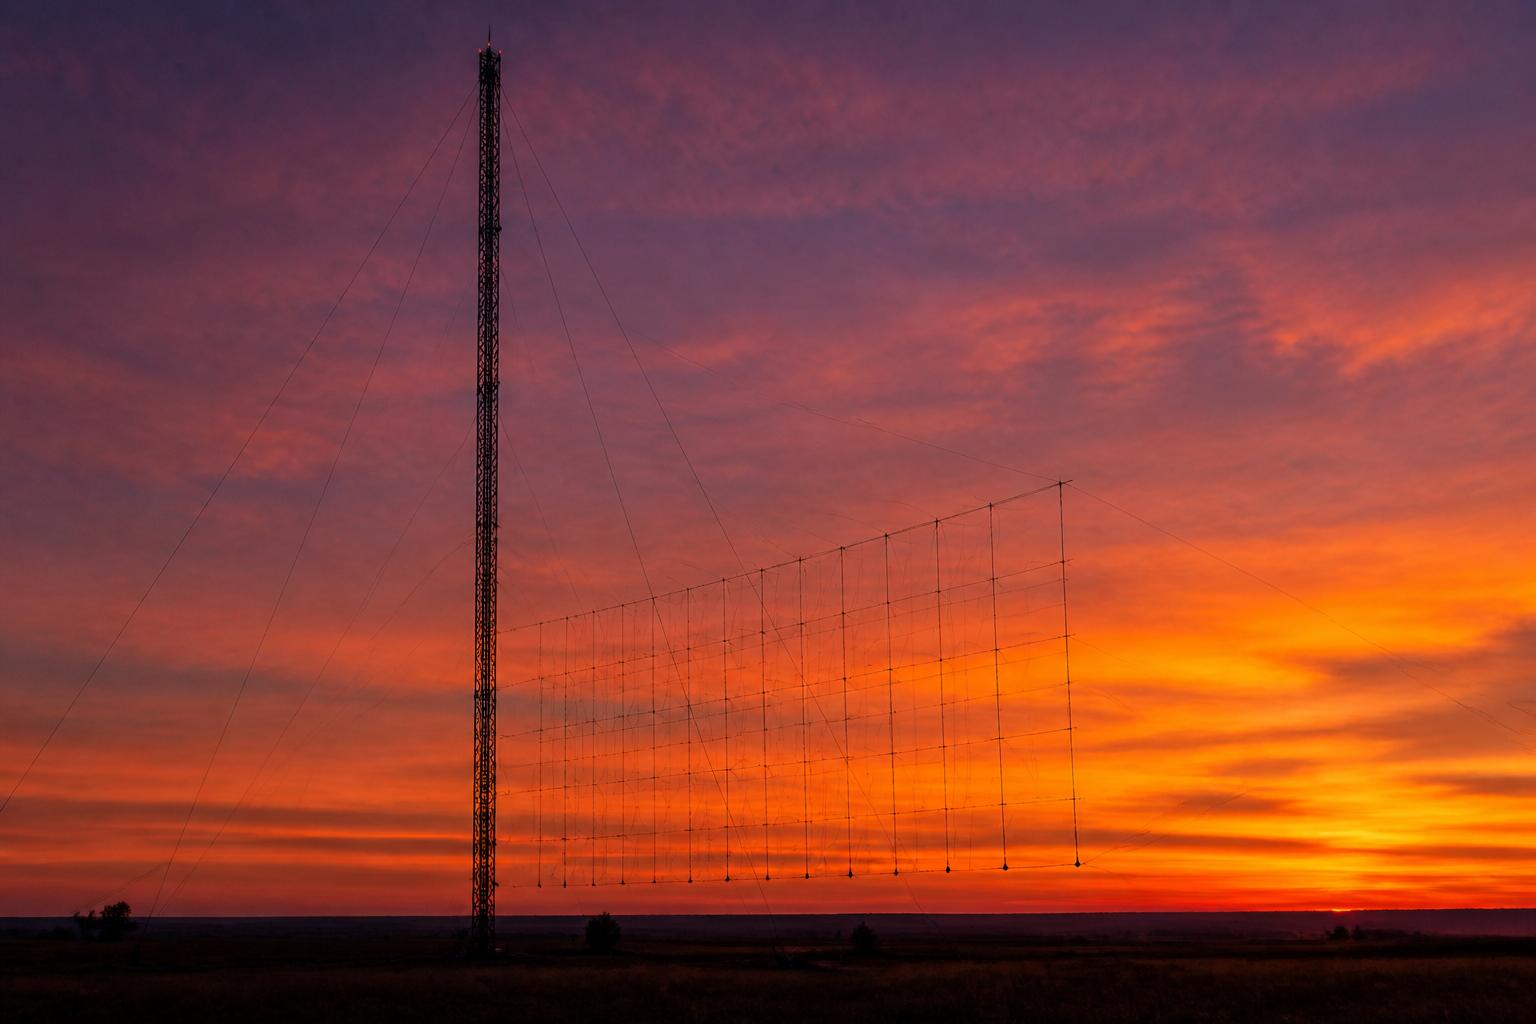
\includegraphics[width=0.58\linewidth]{images/book4/ai/b4-14-shortwave-antenna-sunset.png}

{\small साँझ में कोई लघुतरंग प्रेषण केंद्र: उसकी तरंगें, आयनमंडल की \omterm{def:b2:waves-in-media:plasma}{प्लाज़्मा आवृत्ति} से कुछ मेगाहर्ट्ज़ नीचे, हज़ार किलोमीटर दूर ज़मीन पर लौट आने ही वाली हैं।}
\end{omfigure}

\begin{omfigure}
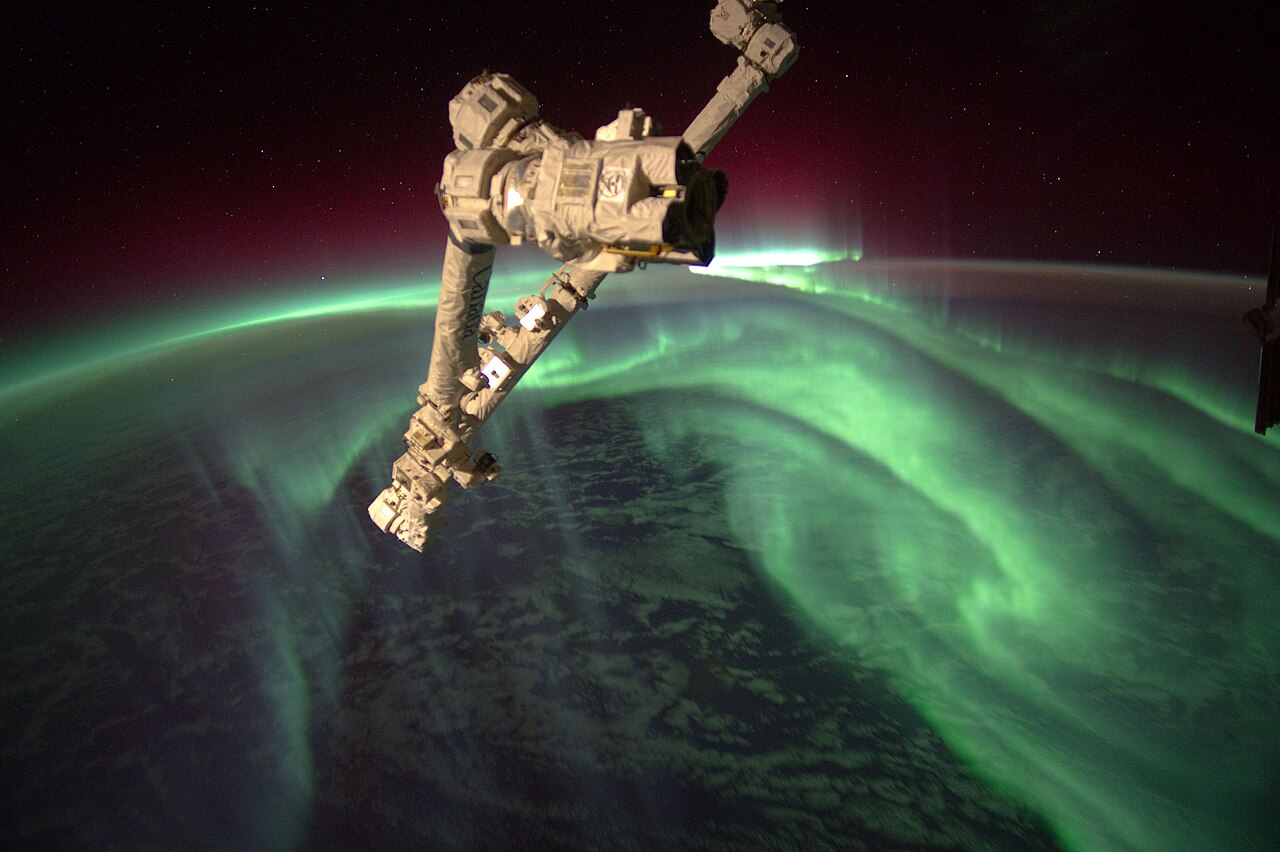
\includegraphics[width=0.6\linewidth]{images/book4/aurora-australis-iss.jpg}

{\small अंतरराष्ट्रीय अंतरिक्ष स्टेशन से खींची गई दक्षिणी ध्रुवप्रभा: सूर्य से आए कण, पृथ्वी के चुंबकीय क्षेत्र से निर्देशित होकर, ऊपरी वायुमंडल के \omterm{def:b2:waves-in-media:plasma}{प्लाज़्मा} को उत्तेजित करते हैं --- वही आयनमंडल जिसकी \omterm{def:b2:waves-in-media:plasma}{प्लाज़्मा आवृत्ति} रेडियो तरंगों को परावर्तित करती है (NASA)।}
\end{omfigure}

\section{समस्या: आयनमंडल, भट्ठी का दरवाज़ा और प्रिज़्म}

\begin{problem}[{सप्ताहांत समस्या --- किसी तरंग की नज़र से तीन पदार्थ: वह
प्लाज़्मा जो GPS संकेतों को मोड़ता है, वह धातु जो सूक्ष्मतरंगों को भीतर रोके
रखती है, और वह काँच जो श्वेत प्रकाश फैला देता है}]
\label{pb:b2:waves-in-media:1}

\medskip
\noindent\textbf{भाग I --- आयनमंडल और GPS।}
F परत में इलेक्ट्रॉन घनत्व $n = \qty{1e12}{m^{-3}}$; और किसी ऊर्ध्वाधर पथ के अनुदिश
इलेक्ट्रॉनों का कुल स्तंभ दिन में $N_T = \int n\,\dd z = \qty{2e17}{m^{-2}}$ है। GPS:
$f_1 = \qty{1575}{MHz}$, $f_2 = \qty{1228}{MHz}$।
\begin{enumerate}
  \item F परत की \omterm{def:b2:waves-in-media:plasma}{प्लाज़्मा आवृत्ति}; क्या GPS पार जाता है? क्या कोई
        \qty{5}{MHz} लघुतरंग?
  \item दिखाइए कि $\omega \gg \omega_p$ के लिए \omterm{prop:b2:dispersion-wave-packets:group}{समूह वेग} $v_g \approx c(1 -
        \omega_p^2/2\omega^2)$ है और \omterm{def:b2:dispersion-wave-packets:relation}{कला वेग} $c(1 + \omega_p^2/2\omega^2)$।
  \item परत पार करते GPS संकेत का अतिरिक्त समूह विलंब: दिखाइए
        $\Delta t = \dfrac{e^2}{8\pi^2\varepsilon_0mc}\,\dfrac{N_T}{f^2}$ और उसे $f_1$ के लिए
        निकालिए; और परास त्रुटि $c\,\Delta t$।
  \item अभिग्राही दोनों आवृत्तियाँ काम में लेता है: दोनों विलंबों से वह
        त्रुटि हटा देता है। $N_T$ को $\Delta t_1 - \Delta t_2$ के पदों में लिखिए;
        विलंब के अंतर पर कितनी परिशुद्धता $N_T$ को $1\%$ तक दे देती है?
  \item प्रश्न 3 का विलंब $f_1$ पर कितने अतिरिक्त वाहक चक्रों के
        बराबर है?
  \item वाहक की कला उतनी ही \emph{आगे} बढ़ जाती है जितना
        समूह पीछे पड़ता है: क्यों (दोनों संशोधनों के चिह्न)? वाहक
        चक्र गिनते किसी अभिग्राही के लिए कौन-सा मायने
        रखता है?
  \item रात में $N_T$ दस गुना घट जाता है: किसी एक-आवृत्ति अभिग्राही के
        लिए दिन में और रात में त्रुटि।
  \item कोई सौर ज्वाला D परत (\qty{80}{km}) में $n$ को टक्करों की भरमार के
        साथ \qty{1e10}{m^{-3}} तक उठा देती है: कौन-सी रेडियो सेवाएँ
        चोट खाती हैं, और GPS ज़रा-सा ही क्यों बिगड़ता है?
\end{enumerate}

\medskip
\noindent\textbf{भाग II --- भट्ठी का दरवाज़ा।}
कोटर की दीवारें और दरवाज़े की जाली इस्पात की हैं ($\gamma = \qty{1.0e6}{S/m}$);
जाली के छेद \qty{1.0}{mm} चौड़े हैं, और शीट \qty{0.5}{mm} मोटी;
$f = \qty{2.45}{GHz}$, $P = \qty{800}{W}$।
\begin{enumerate}[resume]
  \item \qty{2.45}{GHz} पर इस्पात में \omterm{def:b2:dispersion-wave-packets:complex}{त्वचा गहराई}; क्या दीवार "मोटी" है?
  \item सतही प्रतिरोध $R_s = 1/\gamma\delta$; दीवारों (\qty{1}{m^2}) पर आयाम
        $H_0 = \qty{30}{A/m}$ के किसी सतही चुंबकीय क्षेत्र के साथ,
        दीवारों में खोई शक्ति, प्रति एकांक क्षेत्रफल $\tfrac12R_sH_0^2$; और
        $P$ का अंश।
  \item $a \ll \lambda$ चौड़ाई के किसी छेद में क्षेत्र चल नहीं सकता (वह छेद
        कटाव से नीचे कोई तरंग-निर्देशिका है, \cref{ch:b2:guided-waves}):
        वह $\eu^{-\pi z/a}$ की तरह क्षय करता है, जैसे-जैसे मोटाई $z$ बढ़ती है।
        \qty{0.5}{mm} की शीट पार करते आयाम का dB में \omterm{def:b2:dispersion-wave-packets:complex}{क्षीणन}।
  \item आप जाली में से देख क्यों पाते हैं (छेद के आकार के सामने
        प्रकाश का तरंगदैर्घ्य) जबकि सूक्ष्मतरंगें बाहर नहीं निकल पातीं?
  \item काँच की खिड़की $\underline\varepsilon_r = 4 - 0.02\iu$ वाला कोई परावैद्युत है:
        अपवर्तनांक, और उसमें तीव्रता की \omterm{def:b2:dispersion-wave-packets:complex}{क्षीणन} लंबाई; क्या
        काँच गरम होता है?
  \item भट्ठी में कोई धातु का काँटा: उसकी नोकों पर क्षेत्र बढ़ जाता है;
        प्रश्न 8 की \omterm{def:b2:dispersion-wave-packets:complex}{त्वचा गहराई} के साथ, $H_0 = \qty{300}{A/m}$ के लिए सतह
        पर धारा-घनत्व आँकिए (सतह पर $j \approx H_0/\delta$ लीजिए)
        और स्थानीय तापन $j^2/\gamma$ --- चिंगारियाँ क्यों?
\end{enumerate}

\medskip
\noindent\textbf{भाग III --- रेडियो आवृत्ति पर तार।}
\qty{13.56}{MHz} की किसी प्रेरण-तापक कुंडली में $a = \qty{0.5}{mm}$ त्रिज्या का कोई
ताँबे का तार ($\gamma = \qty{6e7}{S/m}$) \qty{20}{A} वर्ग-माध्य-मूल ले चलता है।
\begin{enumerate}[resume]
  \item \omterm{def:b2:dispersion-wave-packets:complex}{त्वचा गहराई}; प्रभावी चालक अनुप्रस्थ काट; और दिष्ट के सामने
        \omterm{ex:b2:waves-in-media:skinuses}{प्रत्यावर्ती प्रतिरोध} प्रति मीटर।
  \item कुंडली के तार के प्रति मीटर व्यय शक्ति; और $h = \qty{20}{W/(m^2.K)}$
        की संवहनी शीतलन के साथ तार जिस ताप तक पहुँचेगा।
  \item कुंडली किसी इस्पात के कार्य-खंड में धाराएँ प्रेरित करती है ($\gamma =
        \qty{1e6}{S/m}$, गरम होने पर $\mu_r \approx 1$): वहाँ \omterm{def:b2:dispersion-wave-packets:complex}{त्वचा गहराई};
        प्रेरण-तापन केवल कोई सतही परत क्यों तपाता है, और यह
        गियरों को कठोर करने में कैसे काम आता है?
  \item कुंडली की हानि घटाने के लिए तार की जगह भीतर पानी वाला कोई
        \qty{3}{mm} का ताँबे का नल रख दिया जाता है: नया प्रतिरोध प्रति मीटर;
        क्या नल का भीतरी भाग धारा ले चलता है?
  \item किस आवृत्ति पर ताँबे में \omterm{def:b2:dispersion-wave-packets:complex}{त्वचा गहराई} तार की त्रिज्या के बराबर
        होगी? उससे नीचे "मोटे तार" के सूत्र की जगह कौन-सा
        सन्निकटन आता है?
\end{enumerate}

\medskip
\noindent\textbf{भाग IV --- प्रिज़्म।}
किसी काँच का $n(\lambda) = 1.500 + \qty{5.0e3}{nm^2}/\lambda^2$ है, और उसका अनुनाद
$\lambda_0 = \qty{100}{nm}$ पर है।
\begin{enumerate}[resume]
  \item जाँचिए कि अनुनाद से बहुत नीचे कौशी रूप \omterm{prop:b2:waves-in-media:lorentz}{लोरेंत्स प्रतिरूप} से
        निकलता है, और यह कि $\omega_p^2/\omega_0^2 = n^2(\infty) - 1$: इस काँच के लिए
        $\omega_p^2/\omega_0^2$ और प्रभावी $n$ का मान।
  \item \qty{400}{nm} और \qty{700}{nm} पर अपवर्तनांक तथा \omterm{def:b2:dispersion-wave-packets:relation}{कला वेग};
        \qty{550}{nm} पर समूह अपवर्तनांक; और किसी तंतु में ऐसे काँच के
        \qty{1}{km} पर दोनों रंगों के बीच विलंब।
  \item \qty{550}{nm} के लिए न्यूनतम विचलन पर कोई \qty{60}{\degree} प्रिज़्म:
        विचलन ($n\sin(A/2) = \sin((A + D)/2)$ लीजिए); \qty{400}{nm} और
        \qty{700}{nm} के बीच कोणीय दूरी (अवकलन कीजिए); और \qty{2}{m}
        दूर किसी पर्दे पर वर्णक्रम की चौड़ाई।
  \item काँच \qty{200}{nm} पर अपारदर्शी क्यों है, और यदि लोहे का कोई अंश
        \qty{700}{nm} पर कोई दुर्बल अनुनाद जोड़ दे तो उसका रंग क्या होगा?
  \item लोरेंत्स चित्र में, प्रिज़्म नीले को लाल से अधिक क्यों मोड़ता है?
  \item एक ही सारणी में, F परत, इस्पात, ताँबे और काँच के लिए,
        उनकी कार्यकारी आवृत्तियों पर, $\underline\gamma$ की प्रकृति और तरंग का
        भाग्य लिखिए।
\end{enumerate}
\end{problem}
